\section{Experimental Evaluation}
\label{sec:ilu:eval}
We have extensively tested \sysname's performance characteristics throughout its development.
Here, we present a limited set of its key performance attributes and focus on new insights into FaaS performance.
All our experiments are conducted on a 48 core Intel Xeon platinum 8160 CPU, and we restrict the worker to 32 GB memory, running Ubuntu 20.04 using Rust version 1.67.0 and Tokio library version 1.19.2.
%
We are interested in evaluating latency overheads and \sysname's suitability as a low-jitter research control plane. 
This evaluation focuses exclusively on the performance of the worker, where we think most per-invocation latency improvement opportunities exist.
Many effective load-balancing policies have been published, but their impact on latency is limited to balancing decision time and warm start ratio.
Our stateless controller's overhead is consistent at less than 0.5ms, and we can thus ignore its latency contribution, for ease of exposition.
Our CH-BL based load-balancer maximizes locality and provides 99\% warm starts, and we focus on single-worker performance to remove unnecessary confounding factors.

% \noindent \textbf{Load Generation.}
% To collect benchmarking data and testing Control Plane Overhead for the different functions we generate \emph{closed loop} requests with varying client threads for 30 min each. We calculate the average for normalization of data collected in any other experiment. 

% For testing different Queue Policies we use open loop request generation. 

% \noindent \textbf{System Tweaks.}
% Ilúvatar itself keeps track of the memory usage and can limit number of concurrent requests dispatched to the system. We use Linux CPU Hotplug support to turn off some of the CPU cores to limit the system size. 

% \vspace*{-8pt}
\subsection{Control Plane and Function Performance}
\label{sec:ilu:eval:ovhead}

\begin{figure}
  \centering  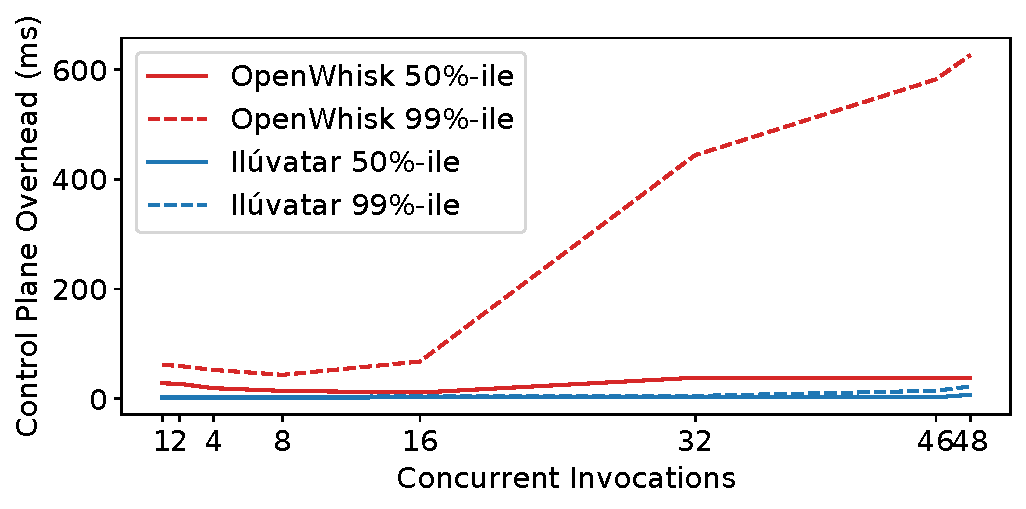
\includegraphics[width=0.6\textwidth]{iluvatar/graphs/scaling/pyaes/overhead-scaling.pdf}
  \caption{The latency overhead of the control plane, as the number of concurrent invocations increases. 
        OpenWhisk overhead is significant and has high variance, resulting in high tail latency. 
        \sysname~reduces this overhead by 100x. }
  \label{fig:ow-scaling}
\end{figure}

\begin{comment}
\begin{figure}
    % Results for pyaes, which has runtime of ~300 ms
    % [0.8, 0.9, 0.99, 0.999, 0.9999, 0.9999]
    % 1 [2.26 2.29 2.40 4.40 4.59 4.59]
    % 2 [2.19 2.24 2.32 3.97 4.74 4.74]
    % 4 [2.28 2.32 3.07 4.81 5.76 5.76]
    % 8 [2.27 2.31 2.48 4.84 12.16 12.16]
    % 16 [2.60 3.02 4.65 7.89 8.66 8.66]
    % 32 [3.18 3.36 4.97 7.91 10.71 10.71]
    % 46 [5.02 6.19 14.50 20.25 26.02 26.02]
    % 48 [12.31 14.89 22.25 28.86 32.52 32.52]
  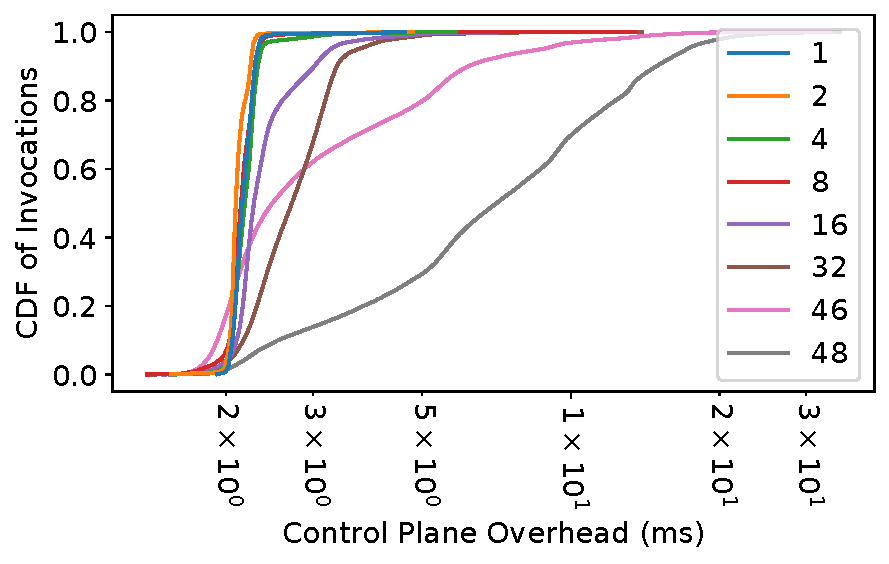
\includegraphics[width=0.6\textwidth]{iluvatar/graphs/scaling/pyaes/overhead-cdf.pdf}
    %  \vspace*{-6pt}
     \caption{\sysname~provides low latency overhead across a range of concurrent invocations.}
        % \vspace*{-6pt}
    \label{fig:ovh-cdf-aes}
\end{figure}
\end{comment}
% Results for lin_pack which has runtime of ~300 microseconds
% Percentiles: [0.8, 0.9, 0.99, 0.999, 0.9999, 0.9999]
% Thread count results (in milliseconds):
% 1 [2.69 3.01 5.68 940.41 956.48 956.48]
% 2 [2.69 2.94 7.12 940.17 942.17 942.17]
% 4 [2.16 2.53 5.74 928.90 935.37 935.37]
% 8 [2.00 2.35 4.78 833.26 860.58 860.58]
% 16 [3.13 3.70 7.05 664.69 709.56 709.56]
% 32 [6.30 7.54 13.78 351.35 430.77 430.77]
% 46 [9.62 11.83 20.14 103.92 15406.05 15406.05]
% 48 [9.64 12.14 20.85 73.48 31507.97 31507.97]

% Results for json_dumps_loads which has runtime of 0.5-1.5 seconds
% [0.8, 0.9, 0.99, 0.999, 0.9999, 0.9999]
% 1 [3.41 3.50 3.87 7.66 10.54 10.54]
% 2 [3.41 3.48 3.99 7.09 12.99 12.99]
% 4 [3.61 3.70 4.20 7.93 8.59 8.59]
% 8 [3.74 3.85 4.81 9.00 15.24 15.24]
% 16 [3.73 3.85 4.27 8.35 15.27 15.27]
% 32 [4.08 4.21 5.15 8.77 15.98 15.98]
% 46 [4.10 4.24 5.27 8.95 15.92 15.92]
% 48 [4.11 4.25 5.17 8.79 16.02 16.02]  

In this subsection, we focus on the latency overheads of \sysname~under different workloads and configurations.
For these experiments, we do not use any queuing, use a single worker, and focus on the most basic \sysname~configuration.  

We start by examining the control plane overheads under a closed-loop load for 30 minutes generated by different number of client threads. 
The control plane overhead CDF for the AES function is shown in Figure~\ref{fig:ow-scaling}. %~\ref{fig:ovh-cdf-aes} 
With 48 concurrent client threads, all the CPUs are fully utilized by function execution. 
Even in this saturated case, the 90 percentile overhead is less than 20ms. 
Just below this saturation limit, with 46 threads, the 90 percentile overhead drops to less than 10ms, and the average is less than 3ms. 

%%%%%%%%%%

\begin{figure*}
  \centering
  \subfloat[PyAES \label{fig:flow:pyaes}] {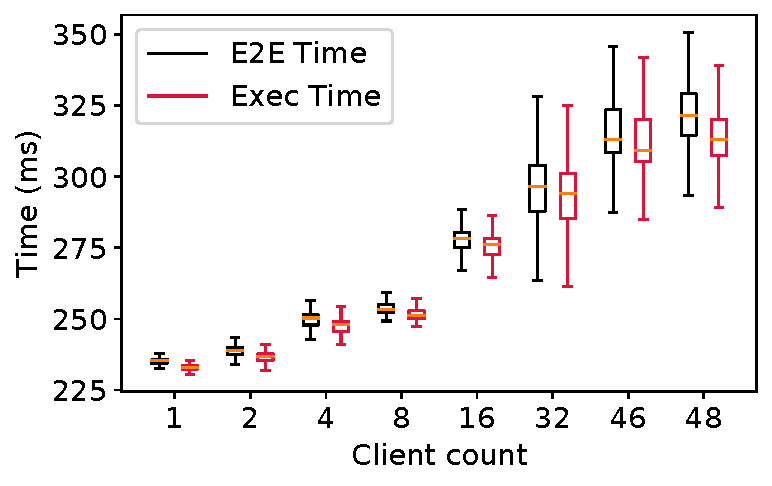
\includegraphics[width=0.3\textwidth]{iluvatar/graphs/scaling/pyaes/worker-e2e-and-exec.pdf}}
    \subfloat[JSON \label{fig:flow:json}] {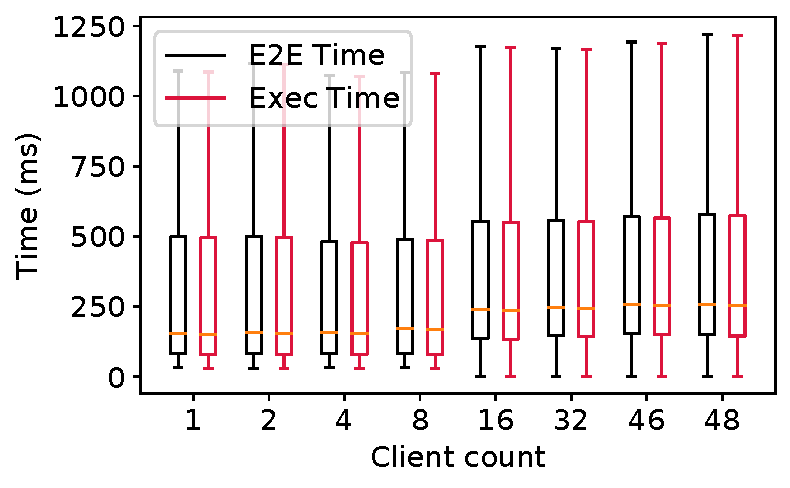
\includegraphics[width=0.3\textwidth]{iluvatar/graphs/scaling/json_dumps_loads/worker-e2e-and-exec.pdf}}
    \subfloat[Video \label{fig:flow:video}] {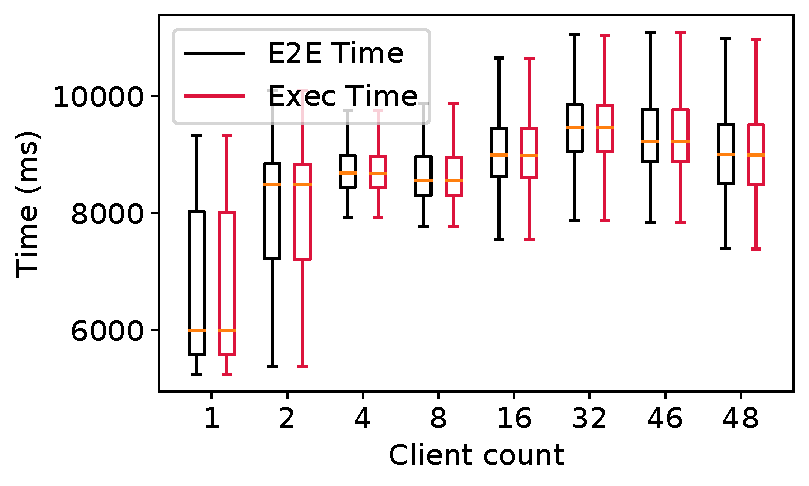
\includegraphics[width=0.3\textwidth]{iluvatar/graphs/scaling/video_processing/worker-e2e-and-exec.pdf}}
      %  \vspace*{-6pt}
      \caption{End-to-end latency and execution times for different functions as we increase the concurrency levels.}
        %  \vspace*{-6pt}
  \label{fig:flow-fn-all}
\end{figure*}

We now provide a more detailed breakdown of the function latency.  
In Figure~\ref{fig:flow-fn-all}, we look at the end to end (E2E) function latency (i.e., flow time) and execution time of different representative functions under different loads.
The flow time is impacted by the control plane overhead and the function code execution time. 
Both these factors are affected by the system load, which in turn is affected by the concurrency level.
% We vary the number of clients invoking the same code in a closed loop, and had each client register the code as a unique function with the system.
The difference between the E2E and the function execution time is the control plane overhead, which is small for all functions and at all load levels.


Interestingly, a significant source of latency variance is the function execution time itself. 
For the small, CPU-intensive PyAES function (Figure~\ref{fig:flow:pyaes}), the  inter-quartile-range is 60ms, which is 20\% the average execution time.
Both the execution time (and hence the E2E latency) and the variance also increases with the system load.
%
This variance is also determined by the non-determinism in the function code.
For instance, the JSON function (Figure~\ref{fig:flow:json}) parses a random json file on every invocation, and thus has a higher natural variance in its execution time.
%
Finally, the video processing function is long and CPU intensive: it downloads and converts a video to grayscale. 
This magnifies the CPU contention, and the function latency increases from 6 to 9 seconds under heavy load.
%


The notable increase in execution time for all three functions is a result of  high  CPU cache miss percentage and a reduction in the instructions per cycle (IPC).
%
We also observed poor cache locality with an increasing number of CPU cores. When the same workload was run on half the number of CPUs (by disabling the rest of the CPU cores), the cache miss percentage significantly dropped (by more than 50\%), along with a proportionate reduction in the latency variance.
%
This highlights and emphasizes the deeper architectural challenges of FaaS, which were also shown by~\cite{shahrad_architectural_2019}. 
%We leave the study of the cause of this effect for future work.

\noindent \textbf{Result:} \emph{\sysname~overheads are small even under heavy load. Function code non-determinism and system load have a higher impact on the function execution times. }


%%%%%%%%%%%%%%%%%%%%

\begin{figure}
  \centering
  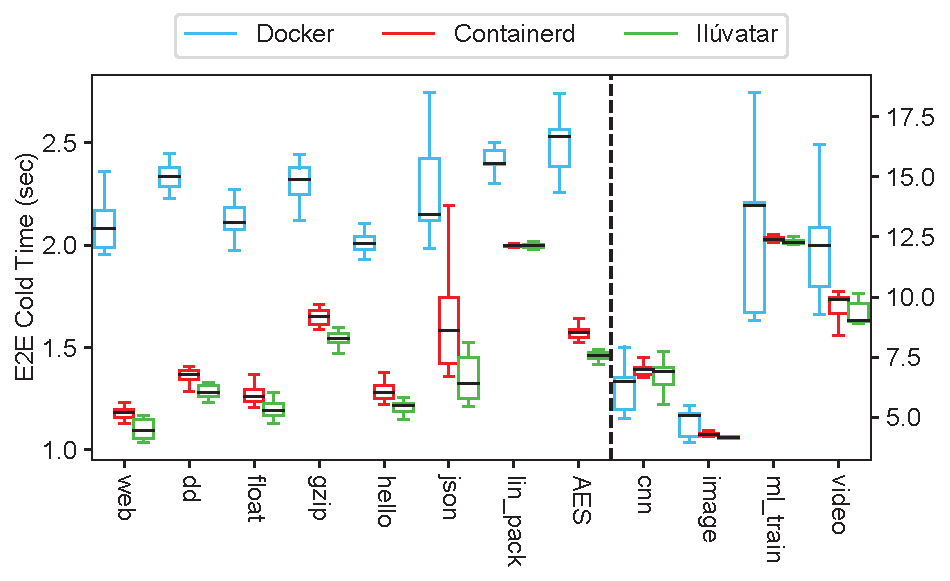
\includegraphics[width=0.6\textwidth]{iluvatar/graphs/impl/benchmark_cold_e2e.pdf}
  % \vspace*{-6pt}
  \caption{Most functions benefit from using a lower-level containerization and OS object caching on cold starts.}
  \label{fig:cold}
  % \vspace*{-6pt}  
\end{figure}

\noindent \textbf{Cold starts.}
So far, we have focused on warm-start performance which dominates function workloads.
\sysname~also incorporates a few optimizations for cold starts. 
Specifically, we are interested in quantifying the impact of the different container backends (containerd and Docker), and the network namespace caching optimizations. 
The end to end cold times for various functions are shown in Figure~\ref{fig:cold}: this includes both container startup time and function initialization overheads. 
In general, smaller functions face a larger impact due to the cold starts, since it represents a higher percentage of their total flow time. 


For small functions (left axis of the figure), using containerd (without network namespace caching) reduces the cold start by more than 40\%, indicating a clear advantage of using a lighter container runtime.
Introducing the namespace caching further reduces the cold start times by 15\% compared to unoptimized containerd which creates a new network namespace for each new container. 
After using the namespace cache, each function invocation sees upwards of $100 ms$ improvement in their cold start time.
%
The effects also hold for larger functions (right axis of Figure~\ref{fig:cold}), where Docker increases both the average and variance of the latency. 

% \vspace*{-8pt}
\subsection{Queuing Performance}
\label{sec:eval:q}

Having seen \sysname~performance in closed-loop micro-benchmarks, we now investigate the impact of its various queuing components and policies.
% We use our open-loop load-generation capabilities described in Section~\ref{sec:impl:support}.
We use an open-loop load-generator, with a random selection of 21 functions from the Azure traces, and pair them with different functions based on their closest running times.
This \quotes{stationary} workload has an average 40 requests per second for 30 minutes. 
This represents an extremely heterogeneous workload in terms of function durations and IATs.
Additionally, we also show results from a \quotes{bursty} workload generated in the same way, but with one function generating a burst of 18 requests per second for one minute.
In this open-loop testing, we prewarm the function containers to prevent excessive cold starts immediately at the start of the workload.
The number of containers to prewarm for each function is determined using Little's law by using their average rates and execution times. 

%~\ref{tab:workload-dsc} lists selected functions and theirs IATs. To test effectiveness of the queue policies we modify the baseline trace to include a burst of function invocation at the rate of 18 request per second in the middle of baseline trace for a window of one minute. Application dd in the table~\ref{tab:workload-dsc} represents it's IAT in bold.
\begin{comment}
\begin{figure}
    \begin{tabular}{|c|c|l|l|}
        \hline
        Application        & \begin{tabular}[c]{@{}l@{}}Benchmark\\ E2E Time (s)\end{tabular} & \begin{tabular}[c]{@{}l@{}}Baseline\\ IATs (s)\end{tabular}                                                       & \begin{tabular}[c]{@{}l@{}}Burst\\ IATs (s)\end{tabular} \\ \hline
        chameleon          & 0.0138       & \begin{tabular}[c]{@{}l@{}}0.076, 0.212, \\ 0.263, 0.391, \\ 0.398, 0.993, \\ 1.527, 3.292, \\ 4.381\end{tabular} & \begin{tabular}[c]{@{}l@{}}0.076, 0.212, \\ 0.263, 0.391, \\ 0.398, 0.993, \\ 1.527, 3.292, \\ 4.381\end{tabular} \\ \hline
        dd                 & 0.105        & \begin{tabular}[c]{@{}l@{}}0.213, 0.501, \\ 5.255, 5.944\end{tabular}                                             & \begin{tabular}[c]{@{}l@{}}\textbf{0.0547}, 0.213, \\ 0.501, 5.255,\\ 5.944,\end{tabular}                                  \\ \hline
        gzip\_compression  & 0.222        & 5.984                                                                                                             & 5.984                                                                                                             \\ \hline
        json\_dumps\_loads & 0.420        & 0.499                                                                                                             & 0.499                                                                                                             \\ \hline
        image\_processing  & 1.969        & 4.043                                                                                                             & 4.043                                                                                                             \\ \hline
        model\_training    & 5.974        & \begin{tabular}[c]{@{}l@{}}2.445, 3.004, \\ 3.746, 5.982, \\ 6.045\end{tabular}                                   & \begin{tabular}[c]{@{}l@{}}2.445, 3.004, \\ 3.746, 5.982, \\ 6.045\end{tabular}                                   \\ \hline
    \end{tabular}%
    \caption{Description of Workloads used for evaluation.}
    \label{tab:workload-dsc}
\end{figure}
\end{comment}

\begin{figure*}
  \centering
  \subfloat[Overcommit \label{fig:q-base:wted}] {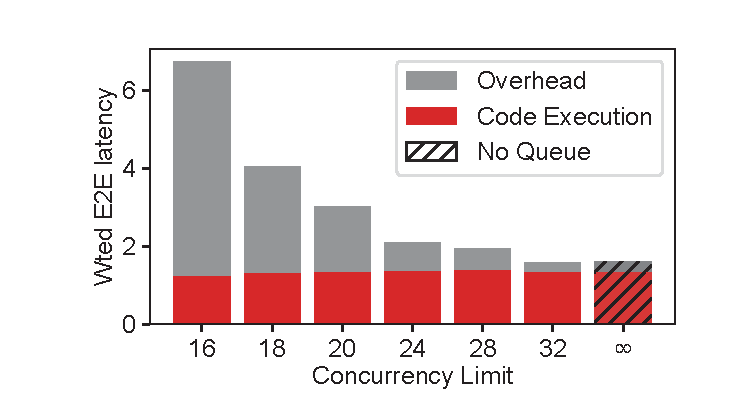
\includegraphics[width=0.3\textwidth]{iluvatar/graphs/old-baseline/breakdown/all_funcs_minheap_ed.pdf}}
  \hfill
  \subfloat[Distribution of function latencies \label{fig:q-base:box}] {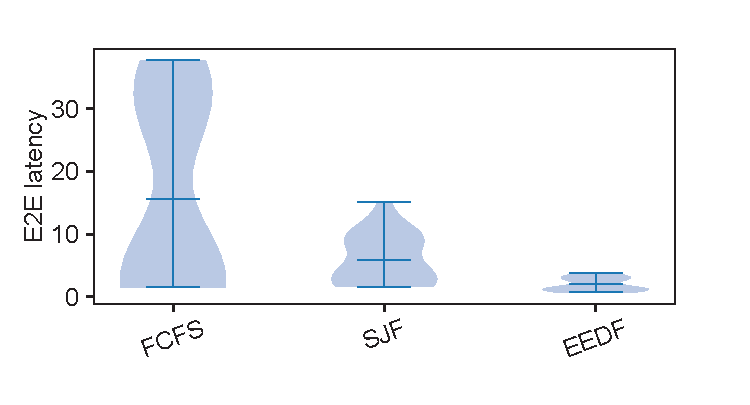
\includegraphics[width=0.3\textwidth]{iluvatar/graphs/scaled_trace2/trace_0_1/violin_e2e_for_each_queue/16_16.pdf}}
  \hfill
  \subfloat[Latency breakdown \label{fig:q-base:breakdown}] {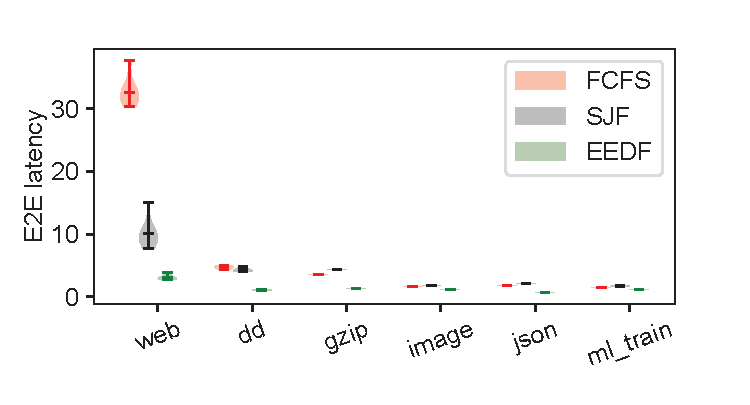
\includegraphics[width=0.3\textwidth]{iluvatar/graphs/scaled_trace2/trace_0_1/violin_func_breakdown/16_16.pdf}}
% \vspace*{-6pt}
  \caption{Queuing performance on the stationary Azure workload. Size-based policies can provide significant latency benefits.}
  \label{fig:q-baseline}
  %  \vspace*{-6pt}
\end{figure*}


\noindent \textbf{Metrics.} 
We use multiple performance metrics to understand and compare different policies.
Since functions can differ in execution time, we always normalize their total latency (flow time) by their execution time in an unloaded system. 
As shown in the previous figures~\ref{fig:flow-fn-all}, even with 1 closed-loop thread, the execution time has variance.
For normalization, we use the \emph{average} execution time with 1 thread for all the functions. 
Second, function popularities can also vary widely. 
We thus compute the \emph{weighted} latency, where each function's normalized latency is weighted by the number of its invocations in the trace.
Thus, the weighted latency represents the latency \emph{per-invocation}. 

\begin{figure}
  \centering 
  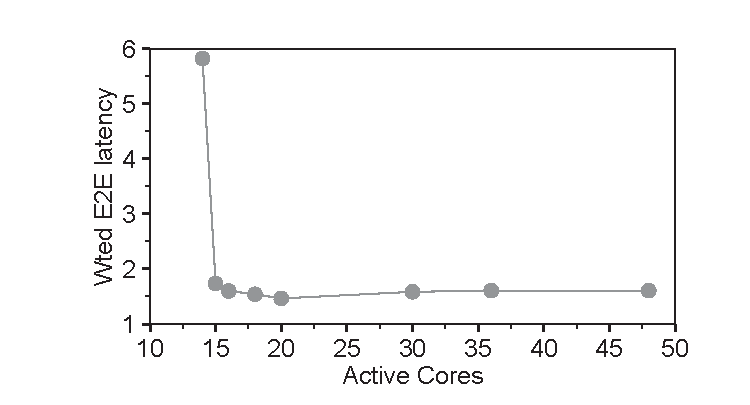
\includegraphics[width=0.6\textwidth]{iluvatar/graphs/scaling/WeakScaling.pdf}
    %  \vspace*{-6pt}
  \caption{The per-invocation function latencies for different system sizes (\# CPUs). We see a sharp inflection point at 16 CPUs, and use that in our queuing evaluation.}
    %  \vspace*{-6pt}
  \label{fig:weak}
\end{figure}


\noindent \textbf{Saturation Testing.}
We are primarily interested in how the queuing impacts the waiting time (which is part of the control plane overhead), and the function performance.
The analysis of queuing is interesting only in saturated scenarios, where there is enough extra load on the system and not all invocations can immediately run on the CPU.
We find this saturation point by weak scaling, and decreasing the number of CPU cores available to \sysname~(by disabling CPU cores using hot-unplug). 
The weighted and normalized latencies for different number of CPUs is shown in Figure~\ref{fig:weak}, which shows the performance \emph{without queuing.}
We see that for our baseline trace, increasing the number of available CPU cores has diminishing returns: the per-invocation latency doesnt benefit when CPUs are increased from 18 to 48.
However, we also see a sharp inflection point at 16 cores: decreasing the size to 14 cores results in a very high, almost $6\times$ slowdown. 
At 16 cores, our workload saturates the system, and we use this system configuration for all our queuing analysis.
We note that the alternative is to scale the workload up and run on on all 48 cores.
However, as we have shown previously through Figure~\ref{fig:flow-fn-all}, the poor hardware locality results in higher variance in the function execution times, and introduces more performance variance.
This variance often masks the control plane jitter, which is of more interest to us. 

% We evaluate our several queuing policies and compare them against a ``no-queue'' policy. 
% When there is no queue to limit concurrency, the control plane must either reject invocations when overloaded or allow resource overcommitment: namely processor sharing.
% Our system chooses the latter and will allow infinite invocations to run concurrently, so long as there is sufficient memory available, we do not overcommit memory.
% This behavior mimics how Openwhisk handles overload scenarios.
\begin{figure*}
  \centering
  \subfloat[Overcommit \label{fig:q-burst:wted}] {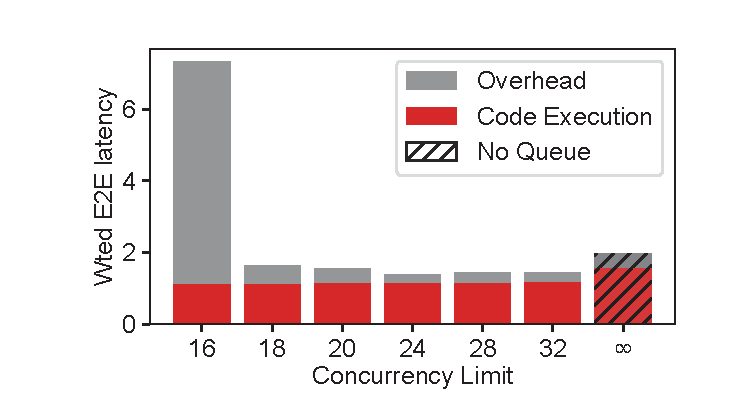
\includegraphics[width=0.3\textwidth]{iluvatar/graphs/scaled_burst_trace2/trace_0_1/barplot_breakdown_perqueue/all_funcs_minheap_ed.pdf}}
  \hfill
  \subfloat[Distribution of function latencies \label{fig:q-burst:box}] {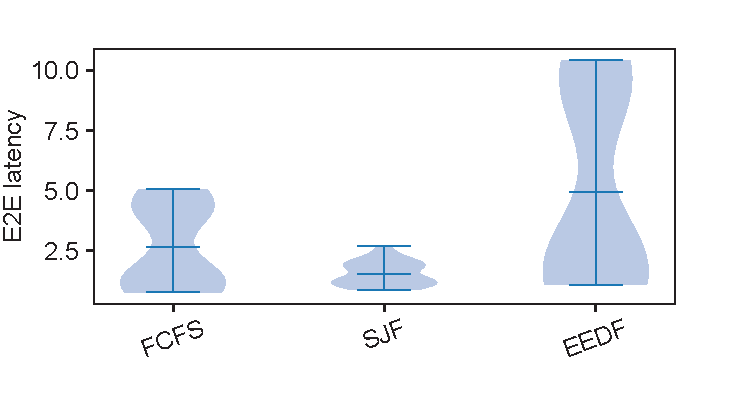
\includegraphics[width=0.3\textwidth]{iluvatar/graphs/scaled_burst_trace2/trace_0_1/violin_e2e_for_each_queue/16_16.pdf}}
  \hfill
  \subfloat[Latency Breakdown \label{fig:q-burst:breakdown}] {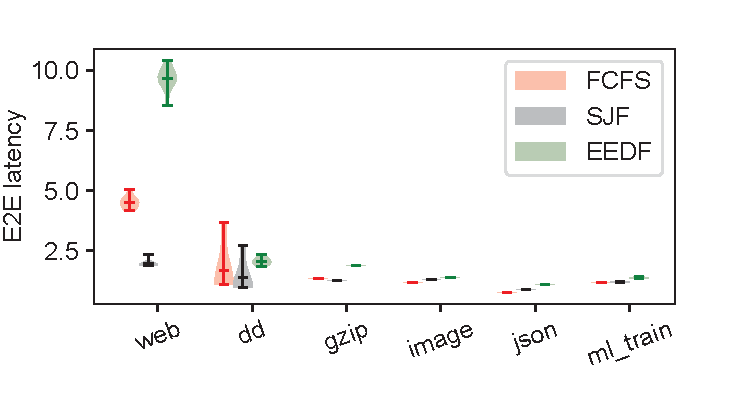
\includegraphics[width=0.3\textwidth]{iluvatar/graphs/scaled_burst_trace2/trace_0_1/violin_func_breakdown/16_16.pdf}}
    %  \vspace*{-6pt}
  \caption{Small and bursty functions can get disproportionately impacted due to queuing. A little overcommitment can go a long way to reduce latency.}
    %  \vspace*{-6pt}
  \label{fig:q-burst}
\end{figure*}

\noindent \textbf{Impact of Overcommitment.}
Many frameworks like OpenWhisk inadvertently overcommit CPUs by running more functions than available CPU cores.
\sysname~can control the degree of overcommitment through its concurrency limit queue regulator.
Figure~\ref{fig:q-base:wted} shows the effect of this overcommitment, when the EEDF (earliest effective deadline) queue policy is used. 
The worker is limited to CPU cores, so higher concurrency limits represent different degrees of overcommitment. 
As the concurrency limit is increased, we see a reduction in the queuing time (which is a major part of the control plane overhead).
For instance, the queuing overhead is negligible when overcommitment level is 2 (i.e., 32 concurrency limit).
However we can see a tradeoff: the increased concurrency risks performance interference, and the code execution time also slightly increases (by 4\%).
For comparison and as a baseline, we also show the \quotes{no queue} configuration which is pure processor sharing and there is no limit on CPU overcommitment.
%
Queuing also reduces cold starts due to concurrent invocations. 
Without queuing, the number of cold starts increased by more than $3\times$. 

For the bursty workload, the impact of overcommitment is even more drastic, as shown in Figure~\ref{fig:q-burst:wted}.
A slight increase in concurrency limit can reduce the weighted latency by more than $3\times$, indicating that overcommitment is more effective for burstier workloads.
Interestingly, the latency improves by $20\%$ with queuing as compared to the \quotes{infinite overcommitment} no queuing case.
This is due to the increase in function execution time due to uncontrolled CPU contention and interference, which the queue helps ameliorate. 

\noindent \textbf{Result:} \emph{CPU overcommitment can reduce queuing times, but come with risk of increased performance interference. \sysname's queue design provides a new effective \quotes{knob} for managing this tradeoff.}

% Bursty here. 

\noindent \textbf{Queuing Policies and Fairness.}
Next, we look at the performance impact of the different queuing policies themselves.
We are interested in the impact on the latencies of the different functions. 
Figure~\ref{fig:q-base:box} shows the normalized latencies of different functions with the different queuing policies.
This scenario has a significant amount of queuing: the concurrency limit is set to 16 (the number of CPUs). 
The function-size aware policies like SJF and EEDF provide much lower latency compared to the standard FCFS: the average latency is reduced by more than $2-3\times$. % 30 to 10 
%The RARE policy prioritizes the highest inter arrival time, and is not size aware, and also tends to suffer under high loads.

A breakdown of the latency of individual functions in Figure~\ref{fig:q-base:breakdown} helps understand this stark performance difference.
The queuing in FCFS increases the total time of the extremely small \quotes{web} function (13ms running time), which increases its latency by $30\times$.
The small-function prioritization by SJF and EEDF reduces this significantly. 

The impact of queuing for the bursty workload is even more interesting, as shown in Figure~\ref{fig:q-burst:box}.
EEDF's average latency is $2\times$ higher than simple FCFS, while SJF is 60\% lower than FCFS. 
Investigating the per-function breakdown again in Figure~\ref{fig:q-burst:breakdown} again points to the contribution of the small web function, which is \emph{also the bursty function}.
The bursty invocations trigger the cold start mitigation, which deprioritizes them, and increases the queuing time, which disproportionately impacts the small functions.
% Bursty here. 

\noindent \textbf{Result:} \emph{Incorporating both function size and arrival times can improve function latency and fairness significantly. Very small functions see a higher \% increase due to queuing.}


%%%%%%%%%%%%%%%%%%%%%%%%%%%%%%


\noindent \textbf{\sysname~vs. Little's law vs. Simulation.}
Finally, we want to show \sysname's suitability for performance modeling, capacity planning, and as a research control plane for developing and evaluating FaaS resource management policies.
We compare the number of concurrent function invocations and queue length (EEDF) with the expected load according to Little's law, computed using average arrival rates and execution times of all functions of our stationary trace. 
We see that the real system metrics, even with all the inherent burstiness in the Azure trace, and the function execution and control plane jitter, are on average very close to the Little's law estimate.
This strongly indicates that our performance is indeed predictable even with highly heterogeneous workloads.

Additionally, Figure~\ref{fig:sim-vs-live-little} also shows the output of our ``simulation'' container backend described in Section~\ref{sec:design:ctr}.
This backend doesn't run actual function code, but exercises all other control plane aspects.
We use constant average function execution times (without accounting for variance and stochasticity) for all invocations.
Even though this simulation setup doesn't capture real-world variability and the impact of server load on function performance, we see that the simulation is also fairly closely aligned with the real experiment output.
This shows that \sysname's integrated simulation framework captures sufficient system dynamics and provides high-fidelity simulations.
This can significantly accelerate FaaS research, especially advances in reinforcement learning based scheduling, which requires high-quality simulations for learning policies. 

\begin{figure}
  \centering
  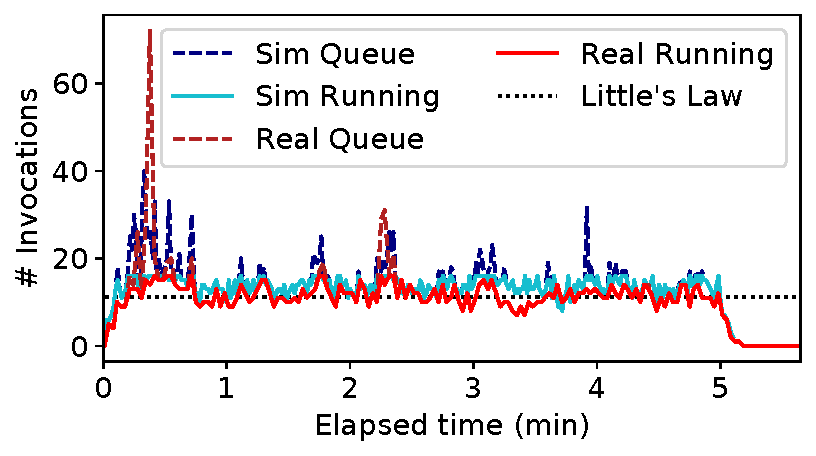
\includegraphics[width=0.6\textwidth]{iluvatar/graphs/trace-compare/baseline/minheap_ed/16/paper-status.pdf}
  \caption{\sysname~running in-silico closely models the in-situ performance. Making it a viable exploration opportunity supplementing real experiments.}
  \label{fig:sim-vs-live-little}
\end{figure}

% \subsection{Scalability}
% \label{sec:eval:scale}

% \textbf{Strong scaling. 48 worse than 16 because of ... bad locality?}

% \textbf{Simulation.}
% FaaS performance highly sensitive to workload due to skewed nature.
% Tough to experiment and report stable outcomes.
% For example, adding one function \emph{decreases} the overall latency. But its due to reporting.

% One way to avoid this is to look into simulations. Lightweight and allow different combinations to be thoroughly explored.

\begin{comment}
\noindent \textbf{Discussion.}
Our worker-centric design allows us to focus on single-worker performance. 
The load balancer is stateless and uses consistent hashing with bounded loads, and has a small overhead of less than 0.5 ms. 
Without workers sharing state (like with OpenWhisk's shared queue), there is no/minimal performance interference, and hotspots are confined in space and time.
%We conjecture that \sysname's performance improvements are largely due to the design and queuing policies for handling invocation bursts. 

Finally, our performance comparison with OpenWhisk is based on end-to-end latency testing. 
Performance tracing of OpenWhisk is challenging due to the highly distributed nature, and the drastically different architectures prevent a clean side-by-side comparison vs. the various components.
The use of Rust vs. Scala provides some performance gains as well, but all our OpenWhisk evaluation was conducted with ample heap sizes to reduce extra garbage collection overheads. 
\end{comment}

\begin{comment}
\begin{figure*}
  \centering
  \subfloat[Overcommit \label{fig:q-base:wted}] {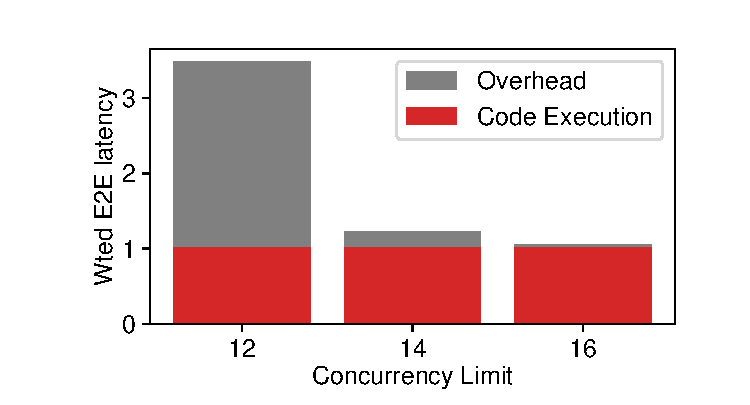
\includegraphics[width=0.3\textwidth]{iluvatar/graphs/simulation/scaled_trace2/trace_0_1/barplot_breakdown_perqueue/all_funcs_minheap_ed.pdf}}
  \hfill
  \subfloat[Distribution of function latencies \label{fig:q-base:box}] {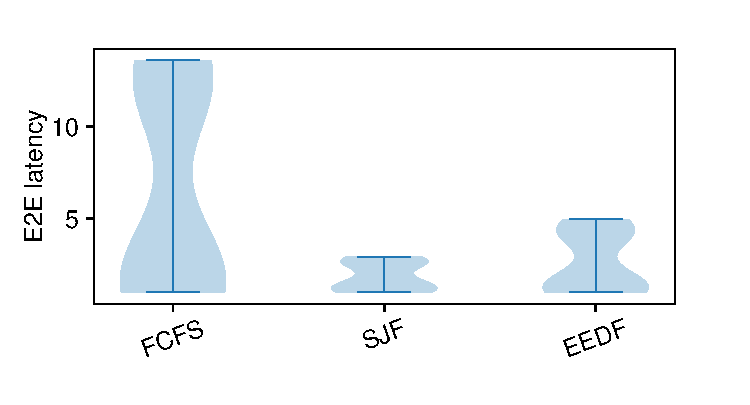
\includegraphics[width=0.3\textwidth]{iluvatar/graphs/simulation/scaled_trace2/trace_0_1/violin_e2e_for_each_queue/16_12.pdf}}
  \hfill
  \subfloat[Code Breakdown \label{fig:q-base:cold}] {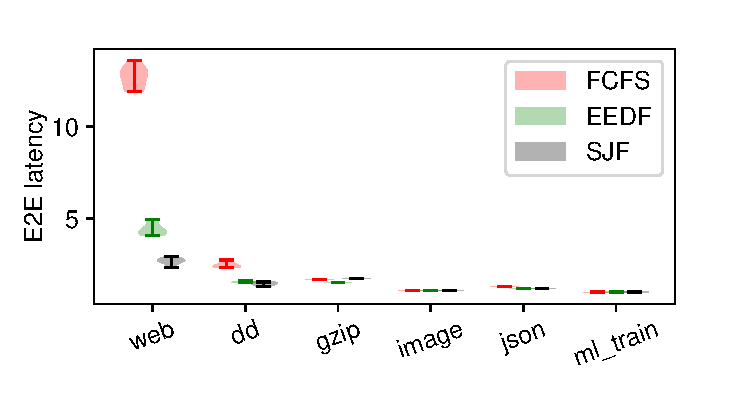
\includegraphics[width=0.3\textwidth]{iluvatar/graphs/simulation/scaled_trace2/trace_0_1/violin_func_breakdown/16_12.pdf}}
 
  % \subfloat[Overcommit \label{fig:q-base:wted}] {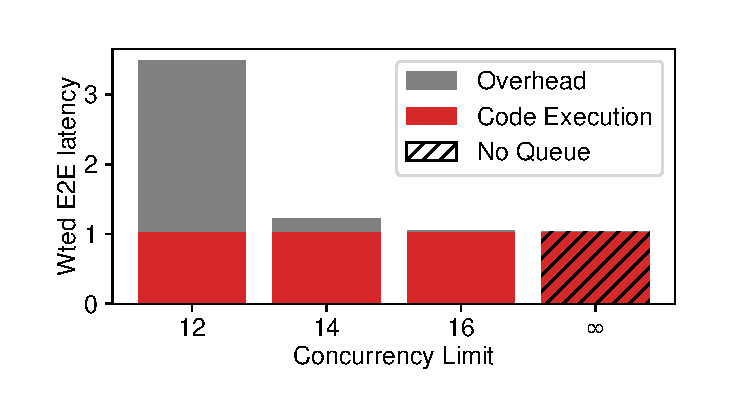
\includegraphics[width=0.3\textwidth]{iluvatar/graphs/burst/breakdown/all_funcs_minheap_ed.pdf}}
  % \hfill
  % \subfloat[Fairness \label{fig:q-base:box}] {\includegraphics[width=0.3\textwidth]{iluvatar/graphs/burst/boxplot/16_24.pdf}}
  % \hfill
  % \subfloat[Cold \label{fig:q-base:cold}] {\includegraphics[width=0.3\textwidth]{iluvatar/graphs/burst/coldstarts/16_24.pdf}}
    % \vspace*{-6pt}
  \caption{Simulation baseline}
  \label{fig:q-burst}
    %  \vspace*{-6pt}
\end{figure*}
\end{comment}

%%% Local Variables:
%%% mode: latex
%%% TeX-master: "paper"
%%% End:
